\documentclass{article}

% if you need to pass options to natbib, use, e.g.:
%     \PassOptionsToPackage{numbers, compress}{natbib}
% before loading neurips_2018

% ready for submission
% \usepackage{neurips_2018}

% to compile a preprint version, e.g., for submission to arXiv, add add the
% [preprint] option:
%     \usepackage[preprint]{neurips_2018}

% to compile a camera-ready version, add the [final] option, e.g.:
\usepackage[preprint]{style}
\usepackage{xcolor}
\usepackage{graphicx}


% to avoid loading the natbib package, add option nonatbib:
%     \usepackage[nonatbib]{neurips_2018}

\usepackage[utf8]{inputenc} % allow utf-8 input
\usepackage[T1]{fontenc}    % use 8-bit T1 fonts
\usepackage{hyperref}       % hyperlinks
\usepackage{url}            % simple URL typesetting
\usepackage{booktabs}       % professional-quality tables
\usepackage{amsfonts}       % blackboard math symbols
\usepackage{nicefrac}       % compact symbols for 1/2, etc.
\usepackage{microtype}      % microtypography
\usepackage{caption}
\usepackage{subcaption}
\usepackage{multirow}
\usepackage{booktabs}


% draft of title 
\title{Reimplementation of Self-Classifier on new datasets
}

% The \author macro works with any number of authors. There are two commands
% used to separate the names and addresses of multiple authors: \And and \AND.
%
% Using \And between authors leaves it to LaTeX to determine where to break the
% lines. Using \AND forces a line break at that point. So, if LaTeX puts 3 of 4
% authors names on the first line, and the last on the second line, try using
% \AND instead of \And before the third author name.

\author{
    Shaochen Bai        \\ \texttt{shaochen@kth.se} \And 
    David Bardvall      \\ \texttt{email} \And 
    Riccardo Periotto   \\ \texttt{periotto@kth.se}
}

\begin{document}
% \nipsfinalcopy is no longer used

\maketitle

\begin{abstract}
% Give an overview of what you have done in the project with the key results and findings of your work. Should be no more than 300 words.
In this work, we re-implement  "Self-Classifier" \cite{self_classifier}, a novel self-supervised end-to-end classification learning approach presented in ECCV 2022. In addition to achieving better performance than its competitors over the self-supervised challenges on different datasets, this approach guarantees additional properties such as scalability, single-stage end-to-end training, and non-degenerate solution. 
We applied the proposed method on MNIST, CIFAR-10, CIFAR-20, and STL-10, achieving 81.90\% clustering accuracy with our best setup for MNIST. 
The original paper is accurate about the mathematical properties of the model and clearly describes the main details of the implementation. Nonetheless, we had to check the provided code and the code of similar methods to set some of the hyperparameters properly. The paper dedicates entire sections to the mathematical proof of the properties of the model and ablation studies. We concentrated our effort on the latter, conducting similar experiments to those reported in the paper and discussing the obtained results. Our code is available on KTH GitHub: \footnote{https://gits-15.sys.kth.se/shaochen/Self-Classifier}.  \\

\textbf{Keywords}: Self-Supervised Learning, Representation Learning, Clustering, Non-contrastive Learning
  
\end{abstract}

\section{Introduction}
% Describe the problem, the approach of the paper, the experiments, and the results. At the high-level talk about what you worked on in your project and why it is important. Then give an overview of your results. 
% + code repository

Many of the most significant results achieved so far by deep learning algorithms come from supervised settings, where the model accesses large amounts of labelled data.
Having labelled datasets is not always guaranteed and is, in any case, less frequent than the possibility of accessing large unlabelled datasets.
The goal of unsupervised learning is to adopt this last category of data. 
As supervised learning, unsupervised learning can be addressed with both generative and discriminative models. For the tasks discussed in our framework (we present them better later), generative models are computationally heavy and discriminative approaches are apparently preferred \cite{byol}. 

The paper focuses on self-supervised learning, which aims to train the model to identify high-level natural features in the data solving a pretext task.
After learning to recognize these features, the model can be used directly or fine-tuned to solve another task (named downstream task) \cite{self_classifier}\cite{swav} \cite{simsiam}\cite{byol}.
The main focus of the literature on self-supervised is to understand the most suitable pretext tasks for specific downstream tasks.
Contrastive learning is the pretext task currently defining the state-of-the-art results \cite{byol}\cite{simclr}. In this task, the idea is to train the model to predict the similarity (or the distance) between two augmented inputs. 
The contrastive learning task is prone to the degenerate solution, where the model maps all the inputs into a single representation. Our paper stands out from the others mainly thanks to the method it presents for dealing with this pitfall.

From a general perspective, the prominent characteristics of Self-classifier are the performance, the high scalability, and the structurally simple single-stage end-to-end approach. These characteristics are also present in other models, but the way Self-Classifier achieves them is doubtless the most compact and straightforward. 

The main contributions of our work are that (i) we compare Self-Classifier and its competitors, summarising the main differences between them \autoref{sec:related_work}; (ii) we reimplemented the proposed model and trained it for datasets different from Imagenet \cite{imagenet}, which is the only one used by the authors ref{sec: data}; (iii) we present the performance achieved by our model and the results obtained through additional ablation studies \autoref{sec:results}.

\section{Related Work}
\label{sec:related_work}
%Discuss the published work related to your project paper, the types of experiments you do and the additional method that you have added to this work or you have compared this paper with (if any).
The current literature on self-supervised learning focuses on the study of pretext tasks and their performances in solving specific downstream tasks. We here better contextualise this framework.

\subsection{Contrastive Learning}
Contrastive learning is just one of the proposed pretext tasks for self-supervised learning. Outside of this category, many other non-contrastive tasks also demonstrated their validity. Some of the most popular non-contrastive pretext tasks adopted are colorization, jigsaw puzzle, image inpainting, relative patch prediction, context prediction, and rotation prediction, just to mention a few \cite{self_classifier}\cite{byol}. The main difference between contrastive and non-contrastive learning lies in the self-generated label that the model aims to predict. In non-contrastive learning, labels correspond to the augmentation applied to the inputs by the model. In contrastive learning instead, labels act as a distance metric between the model's predictions of two different input augmentations. The goal here is to train the model to learn a feature representation which maximises the distances between augmentation of different inputs and minimises those between augmentations of the same data point \cite{byol}. 

Within the contrastive learning category, there is an additional distinction between models trained with negative and positive pairs and those trained using only the positive ones.
Training on both demonstrated to achieve optimal results \cite{simclr}, but the underlying pretext task can sometimes be non-aligned with the downstream one, as described in \cite{self_classifier}. On the other hand, training only on positive pairs is prone to the degenerate solution. 

The architecture at the base of the contrastive learning task is named Siamese network \cite{siamese_network}. Siamese networks are natural tools for comparing two or more input augmentations. In the standard architecture, the different augmentations are fed into a weight-sharing encoder network. In \cite{simsiam} however, they include in the same category also those models that adopt an additional momentum encoder whose weights values are supposed to converge to the same as the trainable network.

% NEED TO CUT SOMETHING UNFORTUNATELY % The last fundamental role in contrastive learning is played by augmentation. Most of the augmenting techniques employed by the models we compared resemble each other, but the original paper refers especially to the ones proposed in \cite{byol}. We present more details on this topic in the methods \autoref{subsec:implementation_details}.

\subsection{Downstream Tasks}
The models we compared to ours for solving the mentioned tasks can be split into two categories: those that only aim to solve representation learning and those that combine, in some way, representation learning and clustering. We highlight that both categories can solve both tasks because: (i) it is always possible to train a cluster on the features obtained from a model of the first category and (ii) it is always possible to access the most informative features of a representation cutting the last layers of a model of the second category. 

Regarding the first category, the authors refer to models such as Exemplar CNN \cite{cnn} e Non-Parametric Instance Discrimination (NPID) \cite{npid}. Their conclusions are that the first does not scale and the second suffers from a lack of consistency across representations stored in the memory bank it adopts \cite{self_classifier}. More recent methods belonging to this same category are MoCo \cite{moco}, BOYL \cite{byol}, SimSiam \cite{simsiam} and DINO \cite{dino}. The main difference between them and Self-Classifier is the way to avoid the degenerate solution. They all implement some sort of stop gradient operation that our model does not need (refer to \autoref{sec:methods}).

The second category includes methods such as DEC \cite{dec}, JULE \cite{jule} and DeepCluster \cite{deepcluster}. The first two are those described by the authors, but they have never been tested on a scale to allow a thorough study of modern ConvNet architectures \cite{deepcluster}. DeepCluster did a step forward, but still, it requires a costly clustering phase and specific precautions to avoid collapsing to trivial solutions \cite{byol}
Again, we better compared Self-classifier with newer models such as SwAV \cite{swav}, Sela \cite{sela}, SCAN \cite{scan} and IIC \cite{iic}, which all share most of the structure we also had to implement. 

What all the modern models from both categories have in common is that they are trained using only positive pairs. As anticipated, this makes them all prone to the degenerate solution and the main differences they have from one another consist in the various strategies implemented to avoid this problem. As in \cite{deepcluster}, we underline that the existence of the degenerate solution is not specific to the unsupervised training, but it is common to any method that jointly learns a discriminative classifier and the labels. Another thing to underline here is that, among the mentioned models, SCAN \cite{scan} and SeLa \cite{sela} are the only ones capable of scaling to large datasets such as ImageNet \cite{imagenet}.

\section{Methods}
\label{sec:methods}
%Describe the original paper's method to the extent that you would need to make your report and findings understandable. Otherwise, here you can describe other methods that you compare with or other methods that you apply on top of what you reimplemented. Here, you also try to justify any methodical modification or incremental changes that you have added to the original paper.It may be helpful to include figures, diagrams, or tables to describe your method or compare it with other methods.
We noted that almost all the components of the proposed architecture appeared in related works. What changes from implementation to implementation are parts of the single component details and how they are combined. This section aims to illustrate the methods adopted in Self-classifier, focusing on the similarities and the differences with the models mentioned in \autoref{sec:related_work}.

\subsection{Avoid the degenerate solution}
\label{subsec:degenerate_solution}
In the following, we compare the techniques for avoiding the degenerate solution when training on positive pairs. In addition to rejecting those techniques based on negative pairs, we also discarded those involving pre-training, memory bank, features post-processing, and cluster reassignment. We did that because, as briefly described in \autoref{sec:related_work}, modern techniques demonstrated to be better.

The paper suggests splitting modern techniques into external clustering, momentum encoder and non-collapsing function. It continues by saying that the principle behind the first two categories is practically the same, so it is possible to identify them together as stop-gradient operations. What distinguishes them is where the stop operation is applied.

External clustering is employed in models that simultaneously learn how to represent and classify the data. We mentioned that the models solving these tasks together most similar to Self-Classifier are SwAV \cite{swav}, Sela \cite{sela} and SCAN \cite{scan}. The difference between these three concerning external clustering is that SwAV and Sela implement it online through a Sinkhorn-Knopp distance algorithm, while SCAN implements it separately using K-means \cite{self_classifier}.

MoCo \cite{moco}, BYOL \cite{byol}, and DINO \cite{dino} do not have a clustering phase and the stop gradient operation is obtained through a second network called momentum encoder. This idea originates from MoCo \cite{moco}, but despite acting as a precursor, this model is slightly different from the others as its training phase employs both positive and negative pairs. 

SimSiam \cite{simsiam} is a step in the direction of simpler models and in better understanding the principles of Siamese networks \cite{simsiam}. It prevents the degenerate problem by applying a stop-grad operation on one of the augmented views. Differently from BYOL \cite{byol} and other models for representation learning, SimSiam directly shares the weights between the branches elaborating the two augmentations. The paper proposing it states that the method can be thought of as “SimCLR without negative pairs” and “SwAV without online clustering” \cite{simsiam}.

The last technique is the most important for the proposed work and involves a non-collapsing function. We include in this technique all the models that solve the problem by defining the loss function or the objective function. The idea of Self-Classifier \cite{self_classifier} is very similar to the one proposed in IIC \cite{iic} as the main point is to define a function that prioritises solutions where the samples are spread among the different classes. IIC does that by defining an objective function which maximises the mutual information between the predictions of two augmented views of the same sample. The loss function proposed by Self-Classifier instead is equivalent to the cross-entropy classification loss under a uniform label prior \cite{self_classifier}. This loss guarantees a non-degenerate, uniformly distributed optimal solution as explained in the original paper \cite{self_classifier}.

% HAD TO CUT
% The idea of uniform partitions is not something new. For example, also SwAV and SeLa's papers claim that their models are constrained to find a "balanced partition for each batch" \cite{swav} and "an equipartition of the data" \cite{sela}. The novelty of Self-Classifier is its simplicity in achieving this property.

In \autoref{fig:1}, we extend the comparison illustrated in \cite{simsiam} to the models we described so far.

\begin{figure}
    \centering
     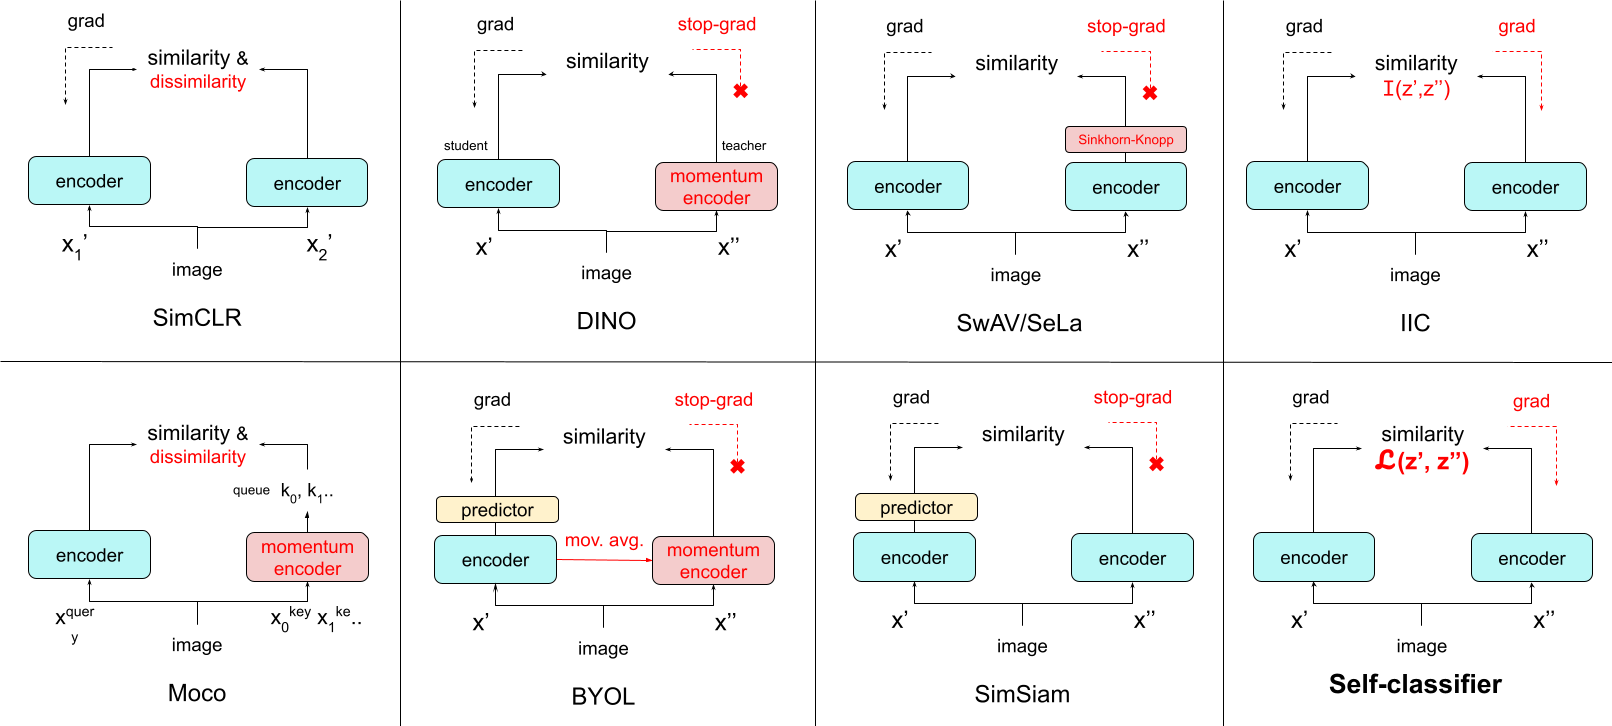
\includegraphics[width=\textwidth]{images/siamese_network_comparison.png}
     \caption{\textbf{Comparison on Siamese architectures.} The illustration starts from the one in SimSiam \cite{simsiam}. We extended it with the main models we described in this document. The difference between each model is highlighted in red and represents how the model solves the degenerate solution problem. The label "dissimilarity" indicates that the model employs negative pairs for training. The dash lines ending with an "X" indicate the presence of a stop gradient operation. The architecture for Self-Classifier is the one on the bottom right. This is similar to the one proposed in ICC \cite{iic} as they are both based on defining a non-degenerate function.}
    \label{fig:1}
\end{figure}

\subsection{Loss function}
The derivation, the mathematical properties and the proofs behind the loss function implemented by Self-Classifier are clearly described in the original paper \cite{self_classifier}. However, for the sake of completeness and given its importance for the model, we report it here below.

\[ 
\begin{array}{cc} 
    l(x_1, x_2) = \sum_{y \in [C]} \frac{p(x_2 | y)}{\sum_{\tilde{y}} p(x_2 | \tilde{y})} \log \left( \frac{N}{C} \frac{p(y | x_1)}{\sum_{\tilde{x}_1} p(y | \tilde{x}_1)} \right)
    &
    \mathcal{L} = \frac{1}{2} \Big( l(x_1, x_2) + l(x_2, x_1) \Big)
\end{array}
 \]


\subsection{Implementation Details}
\label{subsec:implementation_details}

\paragraph{Architecture}
Our architecture follows the same described in the original paper \cite{self_classifier}. This consists of a backbone, followed by a 2-layer MLP with normalisation and a final layer of multiple classification heads. 
Differently from the original paper, we used Resnet-18 instead of Resnet-50 \cite{resnet}. 
We also scaled down the size of the final classification heads (and the final layer for the labelled training) to be proportional to the number of classes in the datasets, keeping the ratio equal to the on in \cite{self_classifier}.

% We use the same architecture as in the original paper (backbone + 2-layer MLP with normalization + multiple classification heads) but appropriately scaled down for our smaller datasets. Mainly, we use Resnet18 instead of Resnet50 for our backbone. Finally, we scale down the size of the final classification heads (and the final layer for the labeled training) to be proportional to the number of classes in the datasets, keeping the ratio equal to the original paper's. 

\paragraph{Image Augmentation}
We used the same augmentations presented in BYOL \cite{byol}, which in turn took them from SimCLR \cite{simclr}\cite{byol}. These augmentations are almost standard in contrastive learning for visual representation and they are used by most of the models we saw. The first augmentation consists in taking a random patch of the image and resizing it. In our implementation, the new dimensions depend on the dataset used. After this, we apply random horizontal flip, colour distortion, Gaussian blur and solarization \cite{byol}. The paper also lists two other augmentations: multi-crop from \cite{swav} and nearest neighbour from \cite{nn_augmentation}. In our model, we implemented the first of these last two techniques.

\paragraph{Optimization} 

\textit{Unsupervised training}.We used a batch size of 512 with softmax temperatures of 0.1 row-wise (over all classes) and 0.05 column-wise (over all batches). We trained the model with the SGD optimizer with a 0.9 momentum and 0.0001 weight decay. The learning rate started at 0.01 and increased linearly to 0.4 within the first 10 epochs. After that, it decreased according to a cosine scheduler over the remaining 790 epochs, reaching a final value of 0.0004.

\textit{Linear training.} We used a batch size of 512. We trained the model with the AdamW optimizer with a momentum of 0.9 and no weight decay. The learning rate started at 0.0004 and decreased toward zero following a cosine scheduler over the 100 epochs of training.

\section{Data and benchmarks}
\label{sec:data}
%Describe the data you are working with for your project. What type of data is it? Where did it come from? How much data are you working with? Did you have to do any preprocessing, filtering, or other special treatment to use this data in your project? If you are using a very standard dataset (Cifar10 etc) then you should focus on describing the state-of-the-art performing methods on the dataset.

% Shaochen version: We compare our obtained results on the standard unsupervised clustering benchmark public available on dataset CIFAR-10\footnote{https://paperswithcode.com/sota/image-clustering-on-cifar-10}, CIFAR-20\footnote{https://paperswithcode.com/sota/unsupervised-image-classification-on-cifar-20?p=improving-unsupervised-image-clustering-with}, STL-10\footnote{https://paperswithcode.com/sota/image-clustering-on-stl-10} and MNIST\footnote{https://paperswithcode.com/sota/image-clustering-on-mnist-full}. The models listed on the benchmarks include SCAN\cite{scan}, SwAV\cite{swav} etc.
We trained our model on common datasets and compared the obtained results with the standard unsupervised clustering benchmarks publicly available. These are: CIFAR-10 \cite{cifar_10}\footnote{https://paperswithcode.com/sota/image-clustering-on-cifar-10}, CIFAR-20\footnote{https://paperswithcode.com/sota/unsupervised-image-classification-on-cifar-20}, STL-10 \cite{stl_10} \footnote{https://paperswithcode.com/sota/image-clustering-on-stl-10} and MNIST \cite{mnist}\footnote{https://paperswithcode.com/sota/image-clustering-on-mnist-full}. 

\section{Experiments and findings}
\label{sec:results}
%Describe and present the experiments that you performed in detail and what is the reason for those experiments. Where applicable define evaluation metrics that you used. Discuss the results that you got. You should include graphs, tables, or other figures to illustrate your experimental results. This is the most important part of your report, be thorough, clear and detailed. Does the reporduction show a significant deviation from those results reported in the original paper? What could be the reason? What extra experiments can you think of to substantiate those speculated reasons? Do the conclusions, observations, statements, and theories of the original paper hold in the new experiments or datasets that you have tried? To what extent? Discuss the similarities and discrepancies and the possible reasonings. 
\subsection{Clustering results}
We evaluated the model on the standard clustering metrics. \autoref{tab:results} illustrates our results. We can not directly compare them to those obtained by the authors, as they trained the model on a different dataset. However, we can compare them with the values from the benchmarks and state that, even if they are significant, they are still far from those obtained by the most performant models. We could have reached better performance by tuning our implementation choices, but the main objective of the review was to show that the model is suitable for what the original paper claims, not to achieve top results. We make this observation also considering the tools and computational power at our disposal.

\begin{table}[h!]
  \caption{Unsupervised image clustering using ResNet-18}
  \label{tab:results}
  \centering
  \begin{tabular}{lcccc}
    \toprule
    Dataset  & NMI    &  AMI     & ARI   & ACC  \\
    \midrule
    MNIST\cite{mnist}   & 83.9427 & 83.9140 & 76.8142 & 81.9000 \\
    CIFAR-10 \cite{cifar_10} & 50.9317 & 50.8450 & 41.5156 & 60.7300 \\
    CIFAR-20 & 30.9210 & 30.4974 & 17.8501 & 32.2400 \\
    STL-10 \cite{stl_10}  & 42.5199 & 42.3921 & 31.6741 & 51.8125	\\
    \bottomrule
  \end{tabular}
\end{table}

\subsection{Linear probing}
Following the linear classification protocol introduced in the original article, we freeze the backbone parameters of the model after the unsupervised training. We then replaced the MLP and head layers with a single linear layer for a 100-epoch supervised training using standard cross-entropy loss. \autoref{fig:linear} reports Top-1 and Top-3 accuracy for the classification performance, where the x-axis indicates the pre-trained epochs of unsupervised learning before linear probing. It is clearly shown in the figure that the quality of representations learned by the model improves with the number of epochs and the linear model converges to a satisfactory state at the end of training. The results of this experiment are compatible with those of unsupervised clustering, which validates the fact that the model simultaneously improves representation learning and clustering performance.

\begin{figure}[hbt!]
     \centering
     \begin{subfigure}[b]{.45\textwidth}
         \centering
         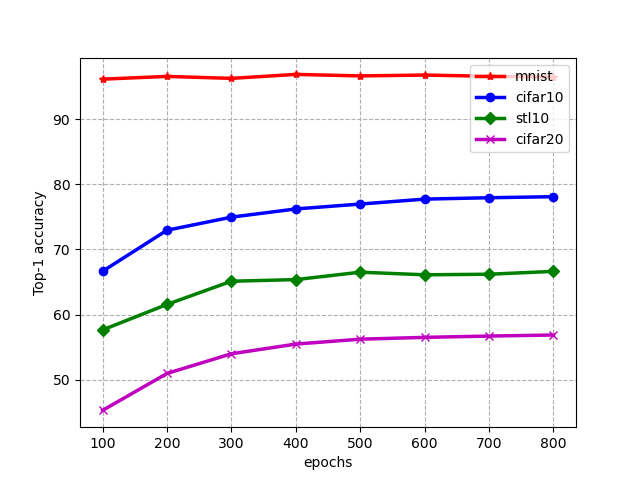
\includegraphics[width=\textwidth]{images/linear_probing_top1.png}
         \caption{Top-1 Accuracy}
         \label{fig:top1}
     \end{subfigure}
     \hfill
     \begin{subfigure}[b]{0.45\textwidth}
         \centering
         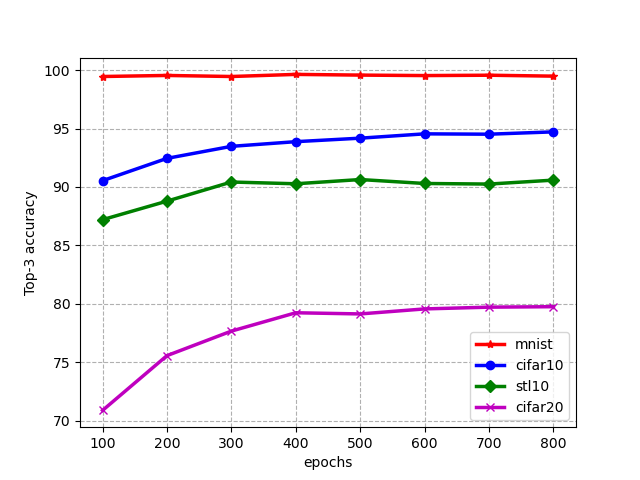
\includegraphics[width=\textwidth]{images/linear_probing_top3.png}
         \caption{Top-3 Accuracy}
         \label{fig:top3}
     \end{subfigure}
     \caption{Linear probing}
     \label{fig:linear}
\end{figure}


\subsection{Qualitative results}
% Paper says: Visualization of High/Low Accuracy Classes Predicted by Self-Classifier
\paragraph{Cluster images visualization} 
% Before: Following the paper, we visualize image samples from both clusters with high accuracy and low accuracy shown in Fig.\ref{fig:visualization}. While it is less obvious to observe miss classified samples from STL-10 benchmark due to its competitive clustering performance, the visualization results in CIFAR-20 show more negative samples. Specifically, in Fig.\ref{fig:low_cifar20}, images of $fox$ and $squirrel$ are clustered together, while they belong to separate classes $medium-sized\ mammals$ and $small\ mammals$ respectively.
Following the paper, we report image samples of clusters with high and low accuracy from different datasets.
As observable in \autoref{fig:visualization}, it is harder to identify miss-classified samples from STL-10 \cite{stl_10}, due to its competitive clustering performance. On the other hand, representations in CIFAR-20 contain more errors. Specifically, \autoref{fig:low_cifar20} shows images of $fox$ and $squirrel$ clustered together, while they belong to separate classes, respectively $medium-sized\ mammals$ and $small\ mammals$.
% I would say: Not a big deal... But we can leave it as it is
\begin{figure}[hbt]
     \centering
     \begin{subfigure}[b]{0.48\textwidth}
         \centering
         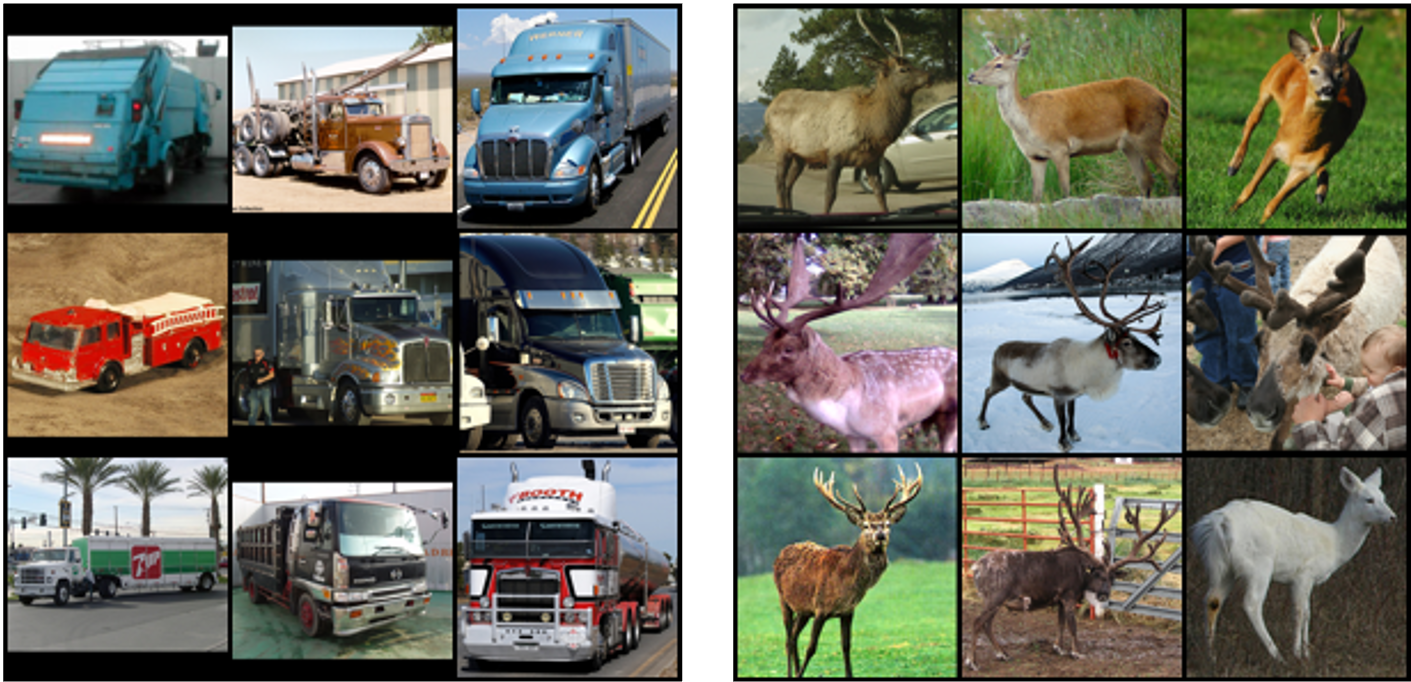
\includegraphics[width=\textwidth]{images/high_accuracy_stl10.png}
         \caption{High accuracy clusters in STL-10}
         \label{fig:high_stl10}
     \end{subfigure}
     \hfill
     \begin{subfigure}[b]{0.48\textwidth}
         \centering
         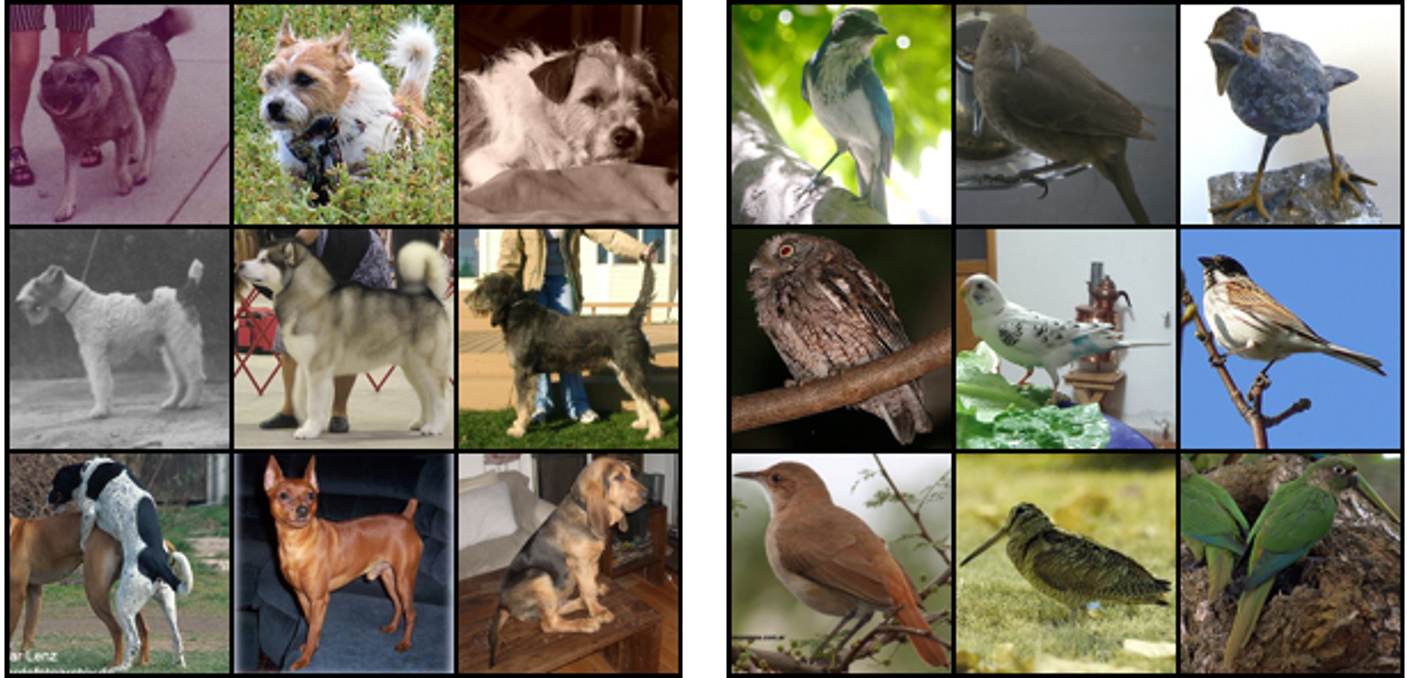
\includegraphics[width=\textwidth]{images/low_accuracy_stl10.png}
         \caption{Low accuracy clusters in STL-10}
         \label{fig:low_stl10}
     \end{subfigure}
     
     \begin{subfigure}[b]{0.48\textwidth}
         \centering
         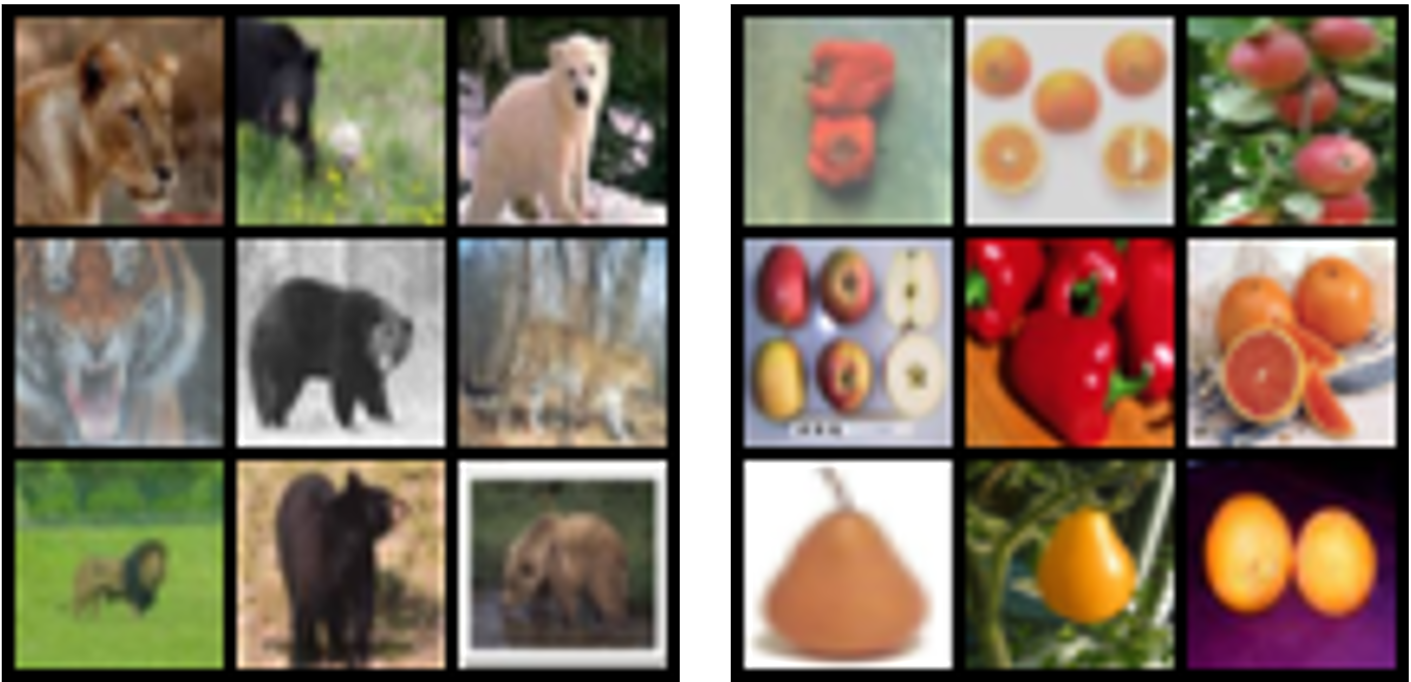
\includegraphics[width=\textwidth]{images/high_accuracy_cifar20.png}
         \caption{High accuracy clusters in CIFAR-20}
         \label{fig:high_cifar20}
     \end{subfigure}
     \hfill
     \begin{subfigure}[b]{0.48\textwidth}
         \centering
         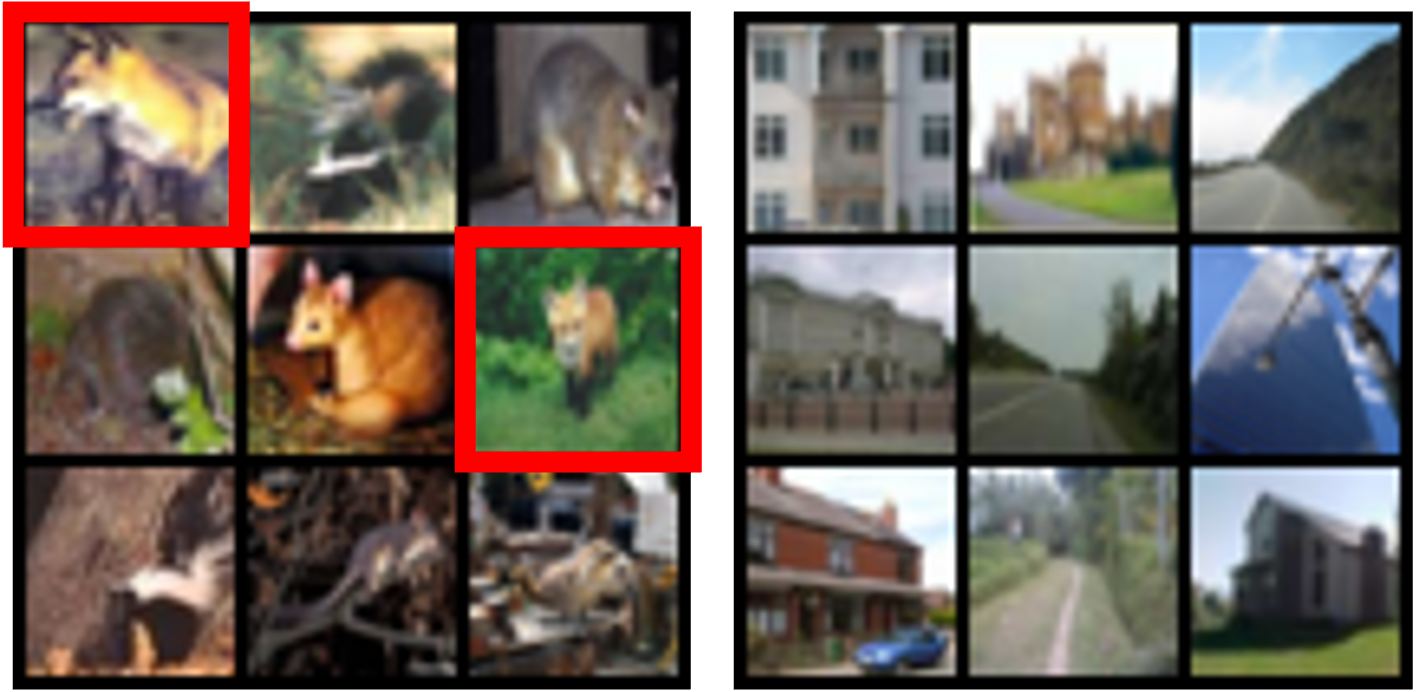
\includegraphics[width=\textwidth]{images/low_accuracy_cifar20.png}
         \caption{Low accuracy clusters in CIFAR-20}
         \label{fig:low_cifar20}
     \end{subfigure}
     \caption{Image visualization for high and low accuracy classes in different datasets }
     \label{fig:visualization}
\end{figure}

\paragraph{Feature visualization with t-SNE}\autoref{fig:t_sne} shows the t-SNE features visualization. It is interesting to note how classes with similar features are close to each other, even in this small two-dimensional space. This result confirms how well the model learns to distinguish the different classes by extrapolating their main features. \autoref{fig:distribution} instead shows how the data samples are distributed among the different classes. In this case, the distribution is not uniform, but the degenerate solution is clearly avoided.

\begin{figure}[hbt!]
     \centering
     \begin{subfigure}[b]{0.45\textwidth}
         \centering
         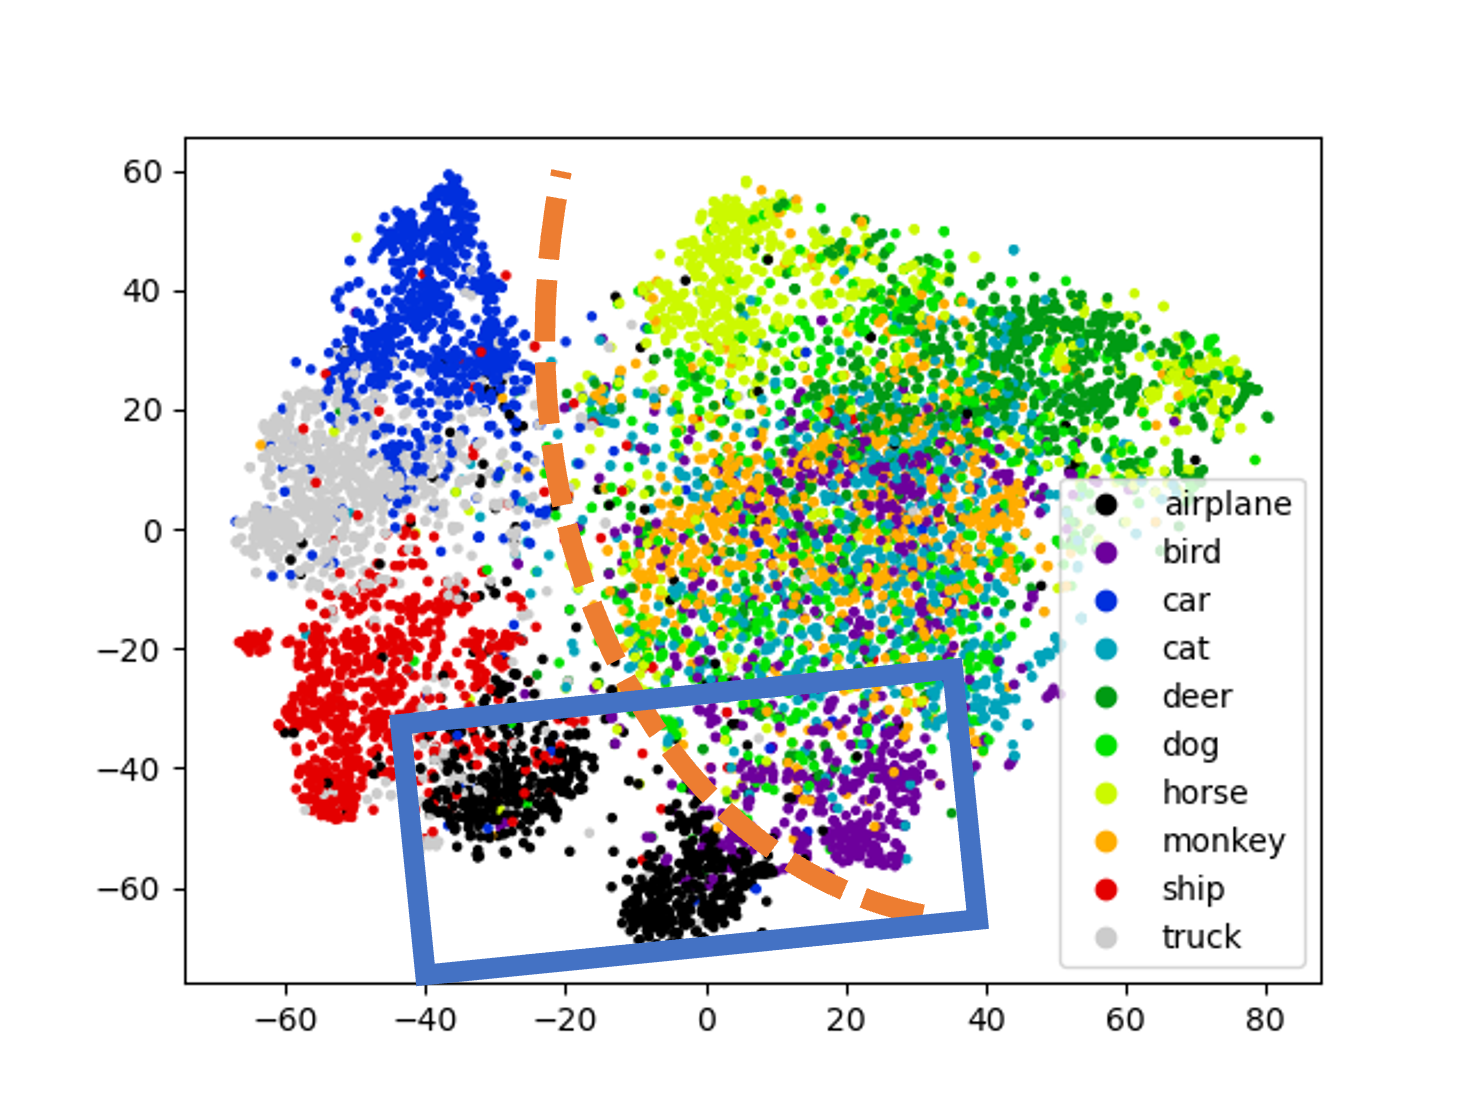
\includegraphics[width=\textwidth]{images/stl10_tsne.png}
         \caption{t-SNE feature visualization}
         \label{fig:t_sne}
     \end{subfigure}
     \hfill
     \begin{subfigure}[b]{0.45\textwidth}
         \centering
         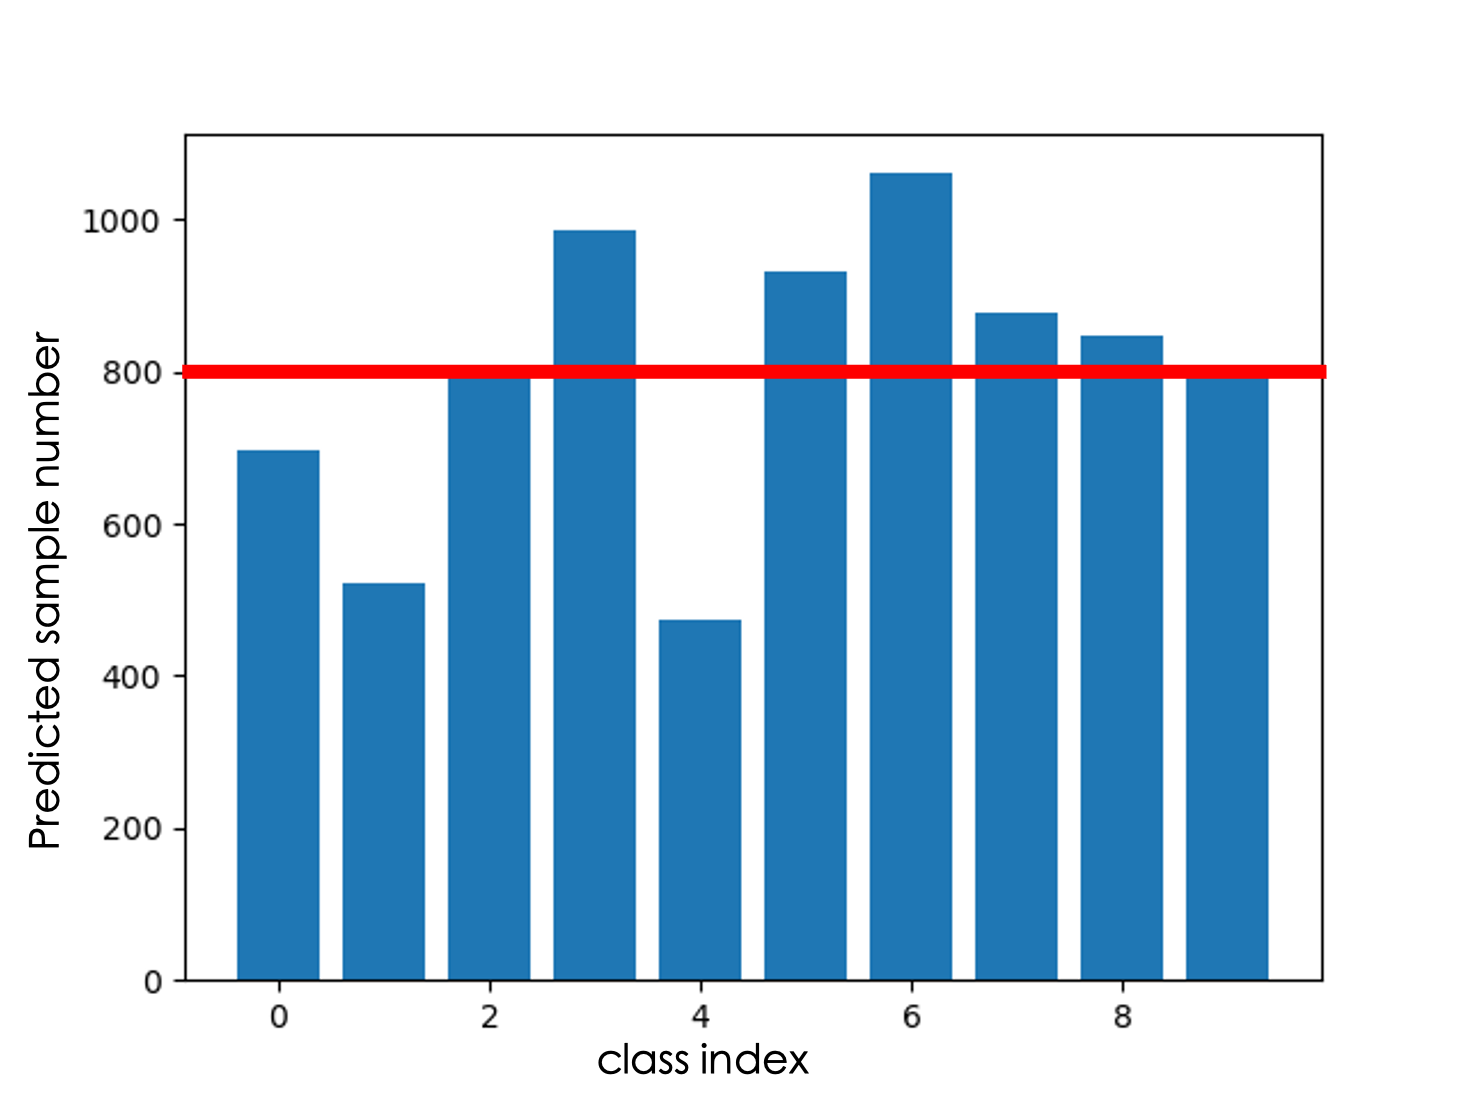
\includegraphics[width=\textwidth]{images/stl10.png}
         \caption{Predicted class number}
         \label{fig:distribution}
     \end{subfigure}
     \caption{Predicted class number}
     \label{fig:combine}
\end{figure}

\subsection{Ablation Study}
% Shaochen:  We focus on the benchmark STL-10 in the ablation study shown in Table.\ref{tab:ablation}, where we compare the base model with model variants that are different in batch sizes, classification head sizes,  temperature settings or multi crop augmentation usage. The results are obtained after 300 epochs following the standard proposed in BYOL\cite{byol}. In general, the proposed method is somewhat robust to different hyper-parameter settings with small performance fluctuations under $5\%$ for NMI and $8\%$ for ACC. We assume ACC suffers more fluctuations because a second step (linear sum assignment) is adopted for unsupervised accuracy calculation. Interestingly, larger batches and more heads do not necessarily lead to better results if we leave the results from the base model. The numbers show $1-4\%$ decrease compared to the smallest configuration which is rather counter-intuitive. We assume that while the loss function expects larger batch size to enforce the uniform priors, small batch size brings about more randomness in the optimization. So there is a trade off between the two properties leading to the final results.
We focused the ablation studies on the STL-10 \cite{stl_10} dataset. \autoref{tab:ablation} shows comparisons between the base model and its variants, which are different in batch sizes, classification head sizes, temperature settings or multi-crop augmentation usage. As in \cite{byol}, we trained the model for 300 epochs for each configuration, as fewer iterations were not achieving stable behaviour. We can state that Self-Classifier is somewhat robust to different hyperparameter settings, with performance fluctuations under $5\%$ for NMI and $8\%$ for ACC. We assume ACC is more subject to oscillations because of the second step (linear sum assignment) adopted for unsupervised accuracy calculation. Interestingly, larger batches and more heads do not necessarily lead to better results. The numbers show a $1-4\%$ decrease in the accuracy when using the largest batch size compared to the smallest, which is quite counterintuitive. We assume that, while the loss function expects a larger batch size to enforce the uniform priors, a small batch size brings more randomness in the optimization. So there is a trade-off between the two properties leading to the behaviour observed.

\begin{table}[htb!]
  \caption{\textbf{Ablation study on unsupervised clustering metrics.} The base model has 512 batch size, $[10,20,40,80]$ head size, and (0.10, 0.05) temperature setting.}
  \label{tab:ablation}
  \centering
  \begin{tabular}{clcccc}
    \toprule
    \multicolumn{2}{c}{Model Variants} & NMI &  AMI & ARI & ACC  \\
    \midrule
    \multirow{3}{*}{Batch Size} & 128 & 39.0715 & 38.9363 & 27.6416 & 48.8500\\
    & 256 & 41.0984 & 40.9675 & 27.3900 & 46.4750\\
    & 1024 & 39.6265 & 39.4921 & 26.2468 & 45.2375 \\
    \midrule
    \multirow{4}{*}{Head Size} & $1*10$ & 39.8843 & 39.7506 &  27.4368 & 48.7750 \\
    & $5*10$  & 38.2264 & 38.0888 & 26.1061 & 47.3250 \\
    & $10*10$ & 38.8565 & 38.7202 & 25.2499 & 44.5375 \\
    & $15*10$ & 39.9663 & 39.8326 & 25.9415 & 44.0750 \\
    \midrule
    \multirow{3}{*}{\shortstack{Temperature\\$(\tau_{row}, \tau_{col})$}} & $(0.07, 0.03)$ & 40.8495 & 40.7174 & 28.4016 & 48.4375 \\
    &$(0.07, 0.05)$ & \textbf{42.5199} & \textbf{42.3921} & \textbf{31.6741} &  \textbf{51.8125}	 \\
    &$(0.10, 0.03)$ & 40.6805 & 40.5485 & 27.7525 & 45.7875 \\
    \midrule
    \multicolumn{2}{c}{Base with Multi-Crop} & 40.5333 & 40.4014 & 25.5025 & 45.0875\\
    \multicolumn{2}{c}{Base} & 40.3517 & 40.2191 & 29.2059 & 50.3375\\
    \bottomrule
  \end{tabular}
\end{table}
    
\section{Challenges}
\label{sec:challenges}
%Challenges you faced when reimplmenting the paper and conducting the experiments. Were all details in the paper? Or did you have to look in the authors code or contact authors to find about some details (you are encouraged to contact the authors)? Was parts of the code quite hard to get them to work as intended? Did you have optimize and tune several hyperparameters? Which ones? Did the framework you used  make the implementation difficult in some ways?
The main challenge in our work is to 
The main things we had to check in the official repository and the code of similar models were the values of some of the hyperparameters (e.g. the dimension of the kernel for the gaussian blur augmentation) and how to implement the image augmentations smartly using PyTorch.
Even looking at the code, we did not implement the last augmentation suggested by the paper. Nevertheless, we believe this is not a relevant problem since its implementation would have overcomplicated the code and the authors do not apply it in their ablation studies. 
The paper also skips a description of how to set up the LARS optimiser and what augmentations to apply when performing linear probing. We had to open the code to get these specifics. To note is that we implemented the LARS optimiser, but it turned out to be worse than AdamW and SGD. According to \cite{simsiam}, this can be because the optimiser is supposed to work better with large batch sizes, which is not our case.
    
\section{Conclusion}
\label{sec:conclusion}
%Summarize your key results - what have you learned? What points do you think one should consider when using the approach of the paper you chose for your project? What can go wrong when reimplementing based on paper and why? A summary of similarities and discrepancies that you found when conducting the experiments. Suggest ideas for future extensions or new applications of your ideas.
In this work, we successfully re-implement Self-Classifier \cite{self_classifier} and explained in detail the peculiarities it has compared to other models designed to solve the same tasks. We demonstrated its capabilities to achieve significant results on different datasets and how it simultaneously solves the features representation and clustering tasks. We presented how similar models deal with the degenerate solution problem and explained why Self-Classifier is revolutionary. 
We do not have anything to add to all the conclusions and limitations the original paper states. The only thing we can not express our argument on is the performance of the model in the new hierarchical alignment metric the paper introduced, as we did not define it for the smaller datasets we used.

% \section{Ethical consideration, societal impact, alignment with UN SDG targets}
%Think and research! Are there any ethical considerations for the original paper, its problem or method, its way of conducting experiments? How about the experiments you did? What societal impact can you imagine about the original paper and its contributions and results? How about your project report? How do you think this paper can push or inhibit the UN SDG targets?

\section{Self Assessment}
%Use the Project Grading Guideline again and assess your project along those guidelines. Argue what grade you think your project deserves and why.
TODO: decide whether to leave it or not


\medskip

\small
\bibliographystyle{plain}
\bibliography{report.bib}

\end{document}
